\chapter{Deriving the Backpropagationg Rule} \label{appendix-a}

%TODO: Fazer a demonstracao do update dos pesos da Neural network. Usar como base \cite{Roth_2016}

\chapter{Proof of Analytic Signal Theorem} \label{appendix-b}

\begin{proof}
Assume $z(t)$ is analytic with a real DC component. Analyticity gives $Z(\omega) = S(\omega) + i\,Y(\omega) = 0$ for $\omega<0$, hence
\begin{equation}
Y(\omega) = i\,S(\omega), \qquad \omega<0. \label{eq:negfreq}
\end{equation}
For $\omega>0$, apply \eqref{eq:negfreq} at $-\omega<0$:
\begin{equation}
Y(-\omega) = i\,S(-\omega). \label{eq:negfreq-applied}
\end{equation}
Taking the complex conjugate of both sides,
\begin{equation}
Y^*(-\omega) = -i\,S^*(-\omega). \label{eq:conjugate}
\end{equation}
Using Hermitian symmetry $Y^*(-\omega) = Y(\omega)$ and $S^*(-\omega) = S(\omega)$ (valid since $y(t), s(t)$ are real),
\begin{equation}
Y(\omega) = -i\,S(\omega), \qquad \omega>0. \label{eq:posfreq}
\end{equation}
Since $y(t)$ is real, $Y(0) \in \mathbb{R}$; likewise $S(0)\in\mathbb{R}$. Hence
\begin{equation}
\mathrm{Im}\{Z(0)\} = \mathrm{Im}\{S(0) + i\,Y(0)\} = Y(0). \label{eq:imz0}
\end{equation}
The real-DC hypothesis $\mathrm{Im}\{Z(0)\}=0$ then forces
\begin{equation}
Y(0) = 0. \label{eq:zerofreq}
\end{equation}
Combining Equations \eqref{eq:negfreq}, \eqref{eq:posfreq}, and \eqref{eq:zerofreq} result in:
\begin{equation}
Y(\omega) = -i\,\mathrm{sgn}(\omega)\,S(\omega) \quad \text{for all } \omega. \qedhere
\label{eq:final}
\end{equation}
\end{proof}


\chapter{Real Signals and TFDs} \label{appendix-c}



\chapter{Spectral Representation Method} \label{appendix-d}



\chapter{An Theoretical Approach for the Dependance of Velocity and Mass} 

In Sections \ref{sec-vel-effect-measurement} and \ref{sec-mass-effect-measurement}, it is shown that the measured accelerations have a dependence with the wagon mass and velocity. In this section, a theoretical approch is presented to explain, in a simplified way, why this dependence exists. Consider, then, a simple model of the wagon represented as a mass-spring-damper system with mass $m$, spring with stiffness $k$ and damper with damping coefficient $c$. Assume, also, that the wagon travels with a constant speed $v$ and the track irregularity is given by $r(\chi)$. Figure \ref{fig:mass-spring-damper} illustrates this model. 
\begin{figure}[H]
    \centering
    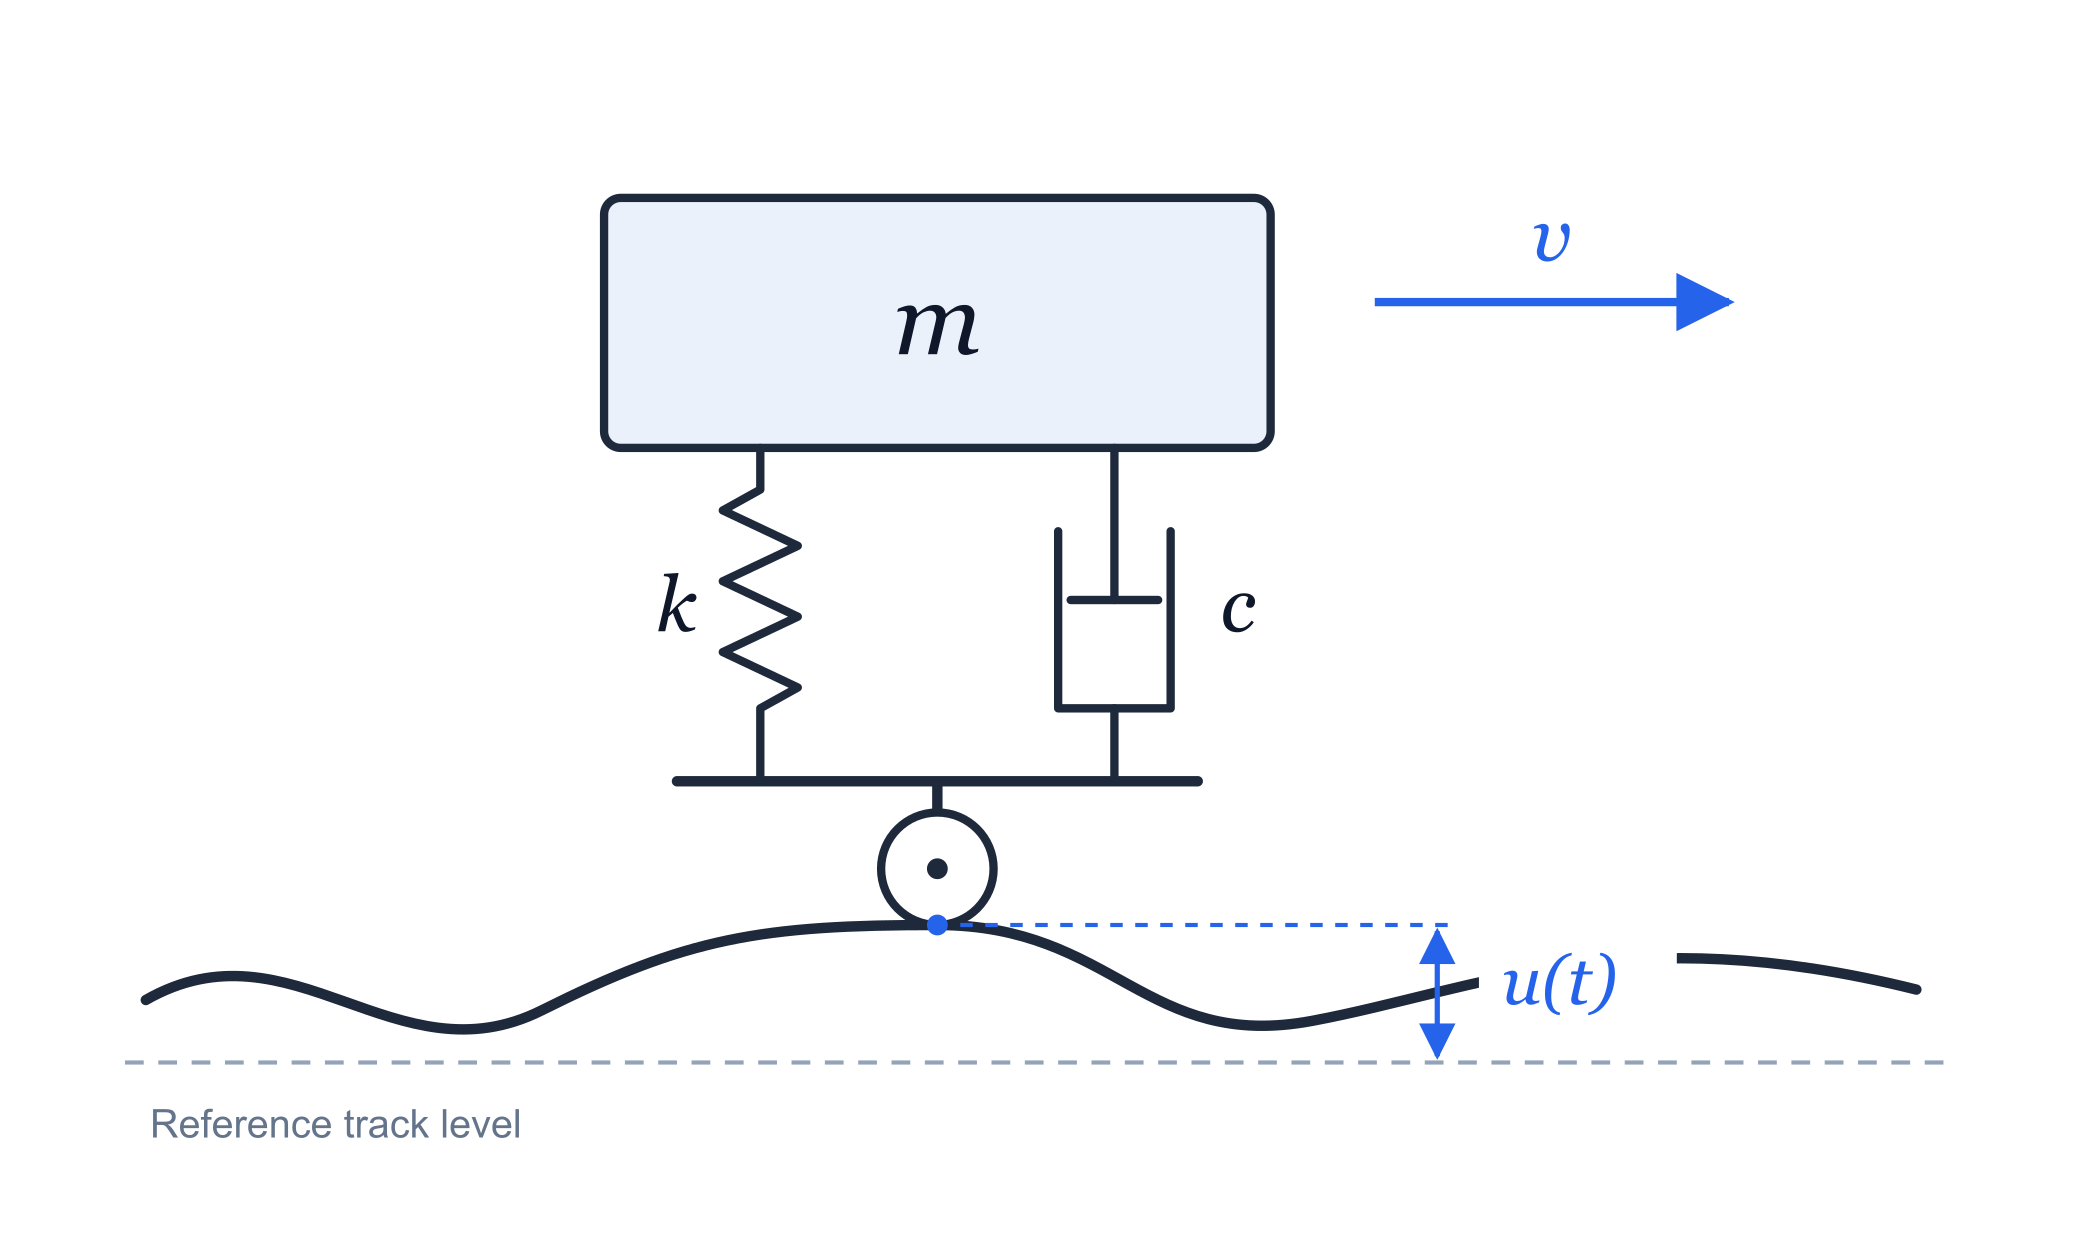
\includegraphics[width=10cm]{Cap3_Methodology/Mass_spring_damper/mass_spring_damper.png}
    \caption{Mass-spring-damper model of the wagon.}
    \label{fig:mass-spring-damper}
\end{figure}

Since the wagon moves at a constant speed $v$, it is possible to define
\begin{equation}
    u(t) = r(\chi (t)) = r(vt)
    \label{eq:spatial-sampling-irregularity}
\end{equation}
where $u(t)$ is the track irregularity as a function of time. Let, then, $z(t)$ be the absolute vertical displacement of the mass, measured from the equilibrium position. The spring force is, then, proportional to the relative displacement $z(t) - u(t)$, and the damping force is proportional to the relative velocity $\dot{z}(t) - \dot{u}(t)$. Using Newton's second law, the equation of motion for the system is:
\begin{equation}
    m \ddot{z (t)} = -k(z(t) - u(t)) - c(\dot{z}(t) - \dot{u}(t))
    \label{eq:equation-of-motion}
\end{equation}
which can be rearranged to give
\begin{equation}
    m \ddot{z (t)} + c \dot{z}(t) + k z(t) = c \dot{u}(t) + k u(t)
    \label{eq:equation-of-motion-rearranged}
\end{equation}
This is just the equation for the base-excited oscillator \cite{newland2005introduction}. Introducing the natural frequency $\omega_n = \sqrt{\frac{k}{m}}$ and the damping ratio $\zeta = \frac{c}{2\sqrt{km}}$, Equation \ref{eq:equation-of-motion-rearranged} can be rewritten as
\begin{equation}
    \ddot{z (t)} + 2 \zeta \omega_n \dot{z}(t) + \omega_n^2 z(t) = 2 \zeta \omega_n \dot{u}(t) + \omega_n^2 u(t)
    \label{eq:normalized-equation-of-motion}
\end{equation}
Since Equation \ref{eq:equation-of-motion-rearranged} is a second order ordinary differential equation with constant coefficients, it admits a frequency-domain solution \cite{peppin1994introduction}. Assume, then, $u(t) = U e^{i \omega t}$ and $z(t) = Z e^{i \omega t}$. Substituting these expressions into Equation \ref{eq:normalized-equation-of-motion} gives:
\begin{equation}
    \left(-m \omega^2 + ic\omega + k\right) Z = \left(ic\omega + k\right)U
\end{equation}
Using this, it is possible to define the displacement transmissibility $H(\omega)$ as:
\begin{equation}
    H(\omega) = \frac{Z}{U} = \frac{k + ic \omega}{k - m\omega^2 + ic \omega}
\end{equation}
Rewriting this in terms of $\omega_n$ and $\zeta$ gives:
\begin{equation}
    H(\omega) = \frac{\omega_n^2 + 2i\zeta \omega_n \omega}{\omega_n^2 - \omega^2 + 2i\zeta \omega_n \omega}
\end{equation}
Defining, then, $x = \frac{\omega}{\omega_n}$, the squared magnitude of the transmissibility can be expressed as:
\begin{equation}
    |H(x)|^2 = \frac{1 + 4 \zeta^2 x^2}{(1 - x^2)^2 + 4 \zeta^2 x^2}
\end{equation}

There are three regimes of interest for the transmissibility. If $x \ll 1$, then $|H(x)|^2 \approx 1$ and the mass follows the track irregularity. If $x \approx 1$, then $|H(x)|^2 \approx \frac{1+4\zeta^2}{4\zeta^2} \approx \frac{1}{4\zeta^2}$ for small $\zeta$, and the body is near resonance. Finally, if $x \gg \max(1, 2\zeta)$, then $1+4\zeta^2 x^2 \approx 4\zeta^2 x^2$ and $(1 - x^2)^2 + 4 \zeta^2 x^2 \approx x^4$, and the transmissibility can be approximated as $|H(x)|^2 \approx \frac{4\zeta^2}{x^2}$. In this last regime, the mass is isolated from the track irregularity.

The above result was derived assuming that the track irregularity profile is a sinusoidal function $u(t) = U e^{i \omega t}$ with a single frequency $\omega$. However, in reality, the track irregularity is modelled as a realisation of a zero-mean stochastic process, containing a wide range of frequencies (Appendix \ref{appendix-d}):
\begin{equation}
    R_r(\xi) = \mathbb{E}[r(\chi) r(\chi + \xi)] = \int_{-\infty}^{\infty} S_r(\omega) e^{i \omega \xi} d\omega
\end{equation}
where $S_r(\omega)$ is the power spectral density of the track irregularity. Using this, the following lemma can be derived:
\begin{lemma}
    If $r(\chi)$ is a wide-sense stationary in space and $u(t) = r(vt)$ with $v >0$ constant, then $u(t)$ is wide-sense stationary in time and
    \begin{equation}
        S_u(\omega) = \frac{1}{v}S_r\left(\frac{\omega}{v}\right)
        \label{eq:lemma}
    \end{equation}
\end{lemma}
The proof of this lemma is given in Appendix \ref{appendix-f}. From this, it is possible to identify one of the effects of the velocity: the argument $\frac{\omega}{v}$ slides the entire track spectrum to higher frequencies as the velocity increases. This means that, as velocity increases, the excited frequencies of the system also increase. 

The solution for the mass-spring-damper system can be written as \cite{newland2005introduction}:
\begin{equation}
    z(t) = \int_{-\infty}^{\infty} h(\theta) u(t - \theta) d\theta
\end{equation}
where $h(t)$ is a real, absolutely integrable impulse response function. Its autocorrelation function is given by
\begin{align}
    R_z(\tau) &= \mathbb{E}\left[\int \int h(\theta_1) h(\theta_2) u(t - \theta_1) u(t + \tau - \theta_2) d\theta_1 d\theta_2\right] \nonumber\\
              &= \int \int h(\theta_1) h(\theta_2) R_u(\tau + \theta_1 - \theta_2) d\theta_1 d\theta_2 
\end{align}
where the expectation operator was moved inside the integral. Taking the FT and using $\mu = \tau + \theta_1 - \theta_2$ gives:
\begin{equation}
    S_z(\omega) = \int \int \int h(\theta_1) h(\theta_2) R_u(\mu) e^{-i\omega(\mu - \theta_1 + \theta_2)} d\mu d\theta_1 d\theta_2
\end{equation}
Since $\mu$, $\theta_1$ and $\theta_2$ are independent variables, the integrals can be separated:
\begin{align}
    S_z(\omega) &= \int h(\theta_1) e^{i\omega \theta_1} d\theta_1 \int h(\theta_2) e^{i\omega \theta_2} d\theta_2 \int R_u(\mu) e^{-i\omega\mu} d\mu  \nonumber \\
                &= H^*(\omega) H(\omega) S_u(\omega)
\end{align}
which gives the result:
\begin{equation}
    S_z(\omega) = |H(\omega)|^2 S_u(\omega)
    \label{eq:PSD-relation}
\end{equation}
Now using that in the frequency domain, the acceleration corresponds to multiplication by $(i\omega)^2$, that is $|H_a(\omega)|=\omega^2 H(\omega)$, and combining Equation \ref{eq:PSD-relation} and \ref{eq:lemma}:
\begin{equation}
    S_{a}(\omega) = \frac{\omega^4}{v}|H(\omega)|^2 S_r\left(\frac{\omega}{v}\right)
    \label{eq:acceleration-temporal-PSD}
\end{equation}
Notice that the left-hand side of this equation is a PSD function of the temporal frequency $\omega$, while the right-hand side is a function of the spatial frequency $\frac{\omega}{v}$. These two PSDs are connected by the operator $K_{t \leftarrow \chi}(\Omega;v,m,k,c) = v^3 \Omega^4|H(\omega)|^2$. In general, it is desirable to have both PSDs in the $\chi$-domain. Define then $a_\chi(\chi) = a(\frac{\chi}{v})$ the acceleration indexed by distance. Its spatial PSD is given by:
\begin{equation}
    S_{a,\chi}(\Omega) = v S_{a}(v\Omega)
\end{equation}
The Fourier Response Function from $r(\chi)$ to $a_\chi(\chi)$ is then given by:
\begin{equation}
    H_{a,\chi}(\Omega) = -(v\Omega)^2 H(v\Omega)
\end{equation}
so that the spatial PSD of the acceleration is given by:
\begin{equation}
    S_{a,\chi}(\Omega) = |H_{a,\chi}(\Omega)|^2 S_r(\Omega) = v^4 \Omega^4 |H(v\Omega)|^2 S_r(\Omega)
    \label{eq:acceleration-spatial-PSD}
\end{equation}
Remember, now, that the variance of a wide-sense stationary process is given by the integral of its PSD over all frequencies, that is:
\begin{equation}
    \sigma^2_{a} = \int_{0}^{\infty} S_{a}(\omega) d\omega = \int_{0}^{\infty} S_{a,\chi}(\Omega) d\Omega =  v^4 \int_{0}^{\infty} \omega^4|H(\omega)|^2 S_r\left(\Omega\right) d\Omega
    \label{eq:variance-acceleration}
\end{equation}
For a specified wavelength band, the PSD can be approximated by a power law, check Section \ref{sec-FRA-Standard}, given by:
\begin{equation}
    S_r(\Omega) = A \Omega^{-w}, \quad \Omega_{min} \leq \Omega \leq \Omega_{max}, \quad 0 < \Omega_{min} < \Omega_{max} < \infty
\end{equation}
For simplicity, assume that the spectrum is approximately zero outside this band. If the spectrum is non-negligible outside this band, their contribution needs to be added to the integral of Equation \ref{eq:variance-acceleration}. Substituting this into Equation \ref{eq:acceleration-spatial-PSD} gives:
\begin{equation}
    S_{a,\chi}(\Omega) = A v^4 \Omega^{4-w} |H(v\Omega)|^2 , \quad \Omega_{min} \leq \Omega \leq \Omega_{max}
\end{equation}
which gives:
\begin{equation}
    \sigma^2_{a} = A v^4 \int_{v\Omega_{min}}^{v\Omega_{max}} \Omega^{4-w} |H(v\Omega)|^2 d\Omega
    \label{eq:variance-acceleration-approx}
\end{equation}
If the contributions of the integral below $v\Omega_{min}$ and above $v\Omega_{max}$ are negligible, then it is possible to approximate the variance as:
\begin{equation}
    \sigma^2_{a} = A v^4 \int_{0}^{\infty} \Omega^{4-w} |H(v\Omega)|^2 d\Omega
    \overset{\Omega = \omega/v}{=} A v^{w-1} \int_{0}^{\infty} \omega^{4-w} |H(\omega)|^2 d\omega = A v^{w-1} I(\omega, \zeta, \omega_n)
\end{equation}
Using this and assuming the vehicle parameters are independent of the velocity:
\begin{equation}
    \sigma_a \propto v^{\frac{w-1}{2}}
\end{equation}
This shows that the variance of the acceleration is a power law function of the velocity, with the exponent depending on the value $w$. In fact, the values of $w$ are limited by the requirement that the integral $I(\omega, \zeta, \omega_n)$ converges. For high frequencies, $|H(\omega)|^2 \approx \frac{4\zeta^2 \omega_n^2}{\omega^2}$, so the integrand becomes:
\begin{equation}
    \omega^{4-w} |H(\omega)|^2 \approx 4\zeta^2 \omega_n^2 \omega^{2-w}
\end{equation}
which is integrable at infinity if $w > 3$. For low frequencies, $|H(\omega)|^2 \approx 1$, and the integrand becomes:
\begin{equation}
    \omega^{4-w} |H(\omega)|^2 \approx \omega^{4-w}
\end{equation}
which is integrable at zero if $w < 5$. Therefore, the exponent $w$ must satisfy $3 < w < 5$.

The influence of the wagon mass, however, is more subtle, as it is embedded within the integral $I(\omega, \zeta, \omega_n)$. It is possible to non-dimensionalize the integral by substituting $\omega = \omega_n x$, which gives:
\begin{equation}
    I(\omega, \zeta, \omega_n) = \int_{0}^{\infty} (\omega_n x)^{4-w} |H(x)|^2 \omega_n dx  = \omega_n^{5-w} \int_{0}^{\infty} x^{4-w} J(\zeta, w) dx
\end{equation}
where
\begin{equation}
    J(\zeta, w) = \int_{0}^{\infty} x^{4-w} \frac{1 + 4 \zeta^2 x^2}{(1 - x^2)^2 + 4 \zeta^2 x^2} dx
\end{equation}
is a pure number that depends only on the damping ratio $\zeta$ and the exponent $w$. Since $\omega_n = \sqrt{\frac{k}{m}}$, $\zeta = \frac{c}{2\sqrt{km}}$, it is possible to write:
\begin{equation}
    \sigma^2_{a} = A v^{w-1} \left(\frac{k}{m}\right)^{\frac{5-w}{2}} J\left(\frac{c}{2\sqrt{km}}, w\right)
\end{equation}
For the wagon mass, the relationship is more complex, as it depends on the integral $J(\zeta, w)$. Two limiting cases will be presented in Sections \ref{sec:lightly-damped-system} and \ref{sec:exact-evaluation-w-4}.

One important observation is that the value of $w$ might change depending on the band $\Omega_{min} \leq \Omega \leq \Omega_{max}$. Which means that the coefficient of the power law might vary for different frequency bands. For example, in the case of $\Omega \gg \Omega_c$ in Equation \ref{eq:FRA-lateral}, the PSd behaves as $S_r(\Omega) \propto \Omega^{-4}$, which does not hold for $\Omega$ values near $\Omega_c$.

\section{Lightly Damped System} \label{sec:lightly-damped-system}

In the case of the lightly damped system, $\zeta \rightarrow 0^+$ the integrand of $J(\zeta, w)$ is dominated by the resonance peak near $x = 1$. In this case, it is possible to approximate $1 - x^2 \approx 2(1 - x)$, $1+4\zeta^2 x^2 \approx 1$, and $x^{4-w} \approx 1$, so that the integrand becomes:
\begin{equation}
    J \approx \int_{0}^{\infty} \frac{dx}{4(1-x)^2 + 4\zeta^2} = \frac{1}{4} \int_{0}^{\infty} \frac{dx}{(1-x)^2 + \zeta^2}
\end{equation}
Substituting $y = 1-x$ gives:
\begin{equation}
    J \approx \frac{1}{4} \int_{-\infty}^{1} \frac{dy}{y^2 + \zeta^2} \approx \frac{1}{4} \int_{-\infty}^{\infty} \frac{dy}{y^2 + \zeta^2} = \frac{\pi}{4\zeta}
\end{equation}
And the variance of the acceleration becomes:
\begin{equation}
    \sigma^2_{a} \approx A v^{w-1} \left(\frac{k}{m}\right)^{\frac{5-w}{2}} \frac{\pi\sqrt{km}}{2c} = \frac{\pi A}{2c} v^{w-1} k^{(6-w)/2} m^{(w-4)/2}
\end{equation}
In this case, the dependence of the mass degenerates into a simple power law, with the exponent depending on the value of $w$:
\begin{equation}
    \sigma_{a} \propto m^{(w-4)/4}
\end{equation} 
This dependence is positive if $w > 4$, that is, the acceleration variance increases with mass, and negative if $w < 4$, and the acceleration variance decreases with mass. In the case $w = 4$, the acceleration variance is independent of the mass. One important observation is that the relative error depends on both $\zeta$ and $w$, and is not uniform in the interval $3 < w < 5$. 

\section{Exact Evaluation at \textit{w} = 4} \label{sec:exact-evaluation-w-4}

For the case $w = 4$, the integral $J(\zeta, w)$ is:
\begin{equation}
    J(\zeta, 4) = \int_{0}^{\infty} \frac{1 + 4 \zeta^2 x^2}{(1 - x^2)^2 + 4 \zeta^2 x^2} dx
\end{equation}
This can be evaluated using the following result:
\begin{equation}
    \int_{-infty}^{infty} \left|\frac{B_0 + i B_1 x}{A_0 + i A_1 x - A_2 x^2}\right| dx = \frac{\pi(B_0^2 A_2+B_1^2 A_0)}{A_0 A_1 A_2}
\end{equation}
Now choosing $A_0 = 1$, $A_1 = 2\zeta$, $A_2 = 1$, $B_0 = 1$, and $B_1 = 2\zeta$, and noticing that the integrand is even, gives:
\begin{equation}
    J(\zeta, 4) = \frac{\pi(1 + 4\zeta^2)}{4\zeta}
\end{equation}
Setting $w = 4$ in Equation \ref{eq:variance-acceleration-approx} gives:
\begin{equation}
    \sigma^2_{a} = A v^3 \left(\frac{k}{m}\right)^{1/2} \frac{\pi(1 + 4\zeta^2)}{4\zeta} = \frac{\pi A}{2c} v^3 \left(k + \frac{c^2}{m}\right)
\end{equation}
In this case, the variance of the acceleration grows with the third power of the velocity, and decreases with the mass, although this effect is much more subtle, as it is embedded within the term $\frac{c^2}{m}$.

It is important to notice that the results derived in this section are much more qualitative than quantitative, as several approximations were made to simplify the analysis. The real model of a wagon is much more complex than the simple mass-spring-damper system presented here, with, for example, multiple degrees of freedom, nonlinearities, and other effects that were not considered. However, the main goal of this section was to show a more theoretical approach to explain the dependence of the acceleration measurements with the wagon mass and velocity.

\chapter{Proof of the E.0.1 Lemma} \label{appendix-f}

\begin{proof}
    From the definition of the autocorrelation function, it is possible to write:
    \begin{equation}
        R_u(\tau) = \mathbb{E}[u(t) u(t + \tau)] = \mathbb{E}[r(vt) r(vt + v\tau)]
    \end{equation}
    Since the mean is constant and the autocorrelation function depends only on $\tau$, $u$ is wide-sense stationary in time. Now, taking the FT and using $\xi = v\tau$:
    \begin{equation}
        S_u(\omega) = \int_{-\infty}^{\infty} R_r(v\tau) e^{-i\omega\tau} d\tau = \frac{1}{v} \int_{-\infty}^{\infty} R_r(\xi) e^{-i\frac{\omega}{v}\xi} d\xi = \frac{1}{v} S_r\left(\frac{\omega}{v}\right)
    \end{equation}
\end{proof}
